\section{Summary of Layers}
\label{sec:layers}
This section summarizes the layers of the mapping tool and their organization. 

\subsection{Feature Types and Visualization Methods}

Layers of the mapping tool fall into one of the following categories: area, highway and point features. Each feature can be visualized as a gradient with respect to an associated attribute. The mechanism for visualizing the gradient varies depending on the type of feature.

\subsubsection{Area Features}
\textit{Area features} represent sets of areal regions separated by boundaries, such as U.S. states. Attributes that can be visualized as with respect to area features include commercial electricity price (visualized by state) and grid emission intensity (visualized by state or by balancing authority). Attributes are visualized by coloring the area of each region using a gradient from white (smallest attribute value) to solid red (largest attribute value). 

Fig. \ref{fig:area_features} shows two sample area features, and the right-hand figure illustrates the use of a color gradient to visualize an area attribute. 

\begin{figure}[ht]
    \centering
    \begin{subfigure}[b]{0.49\textwidth}
        \centering
        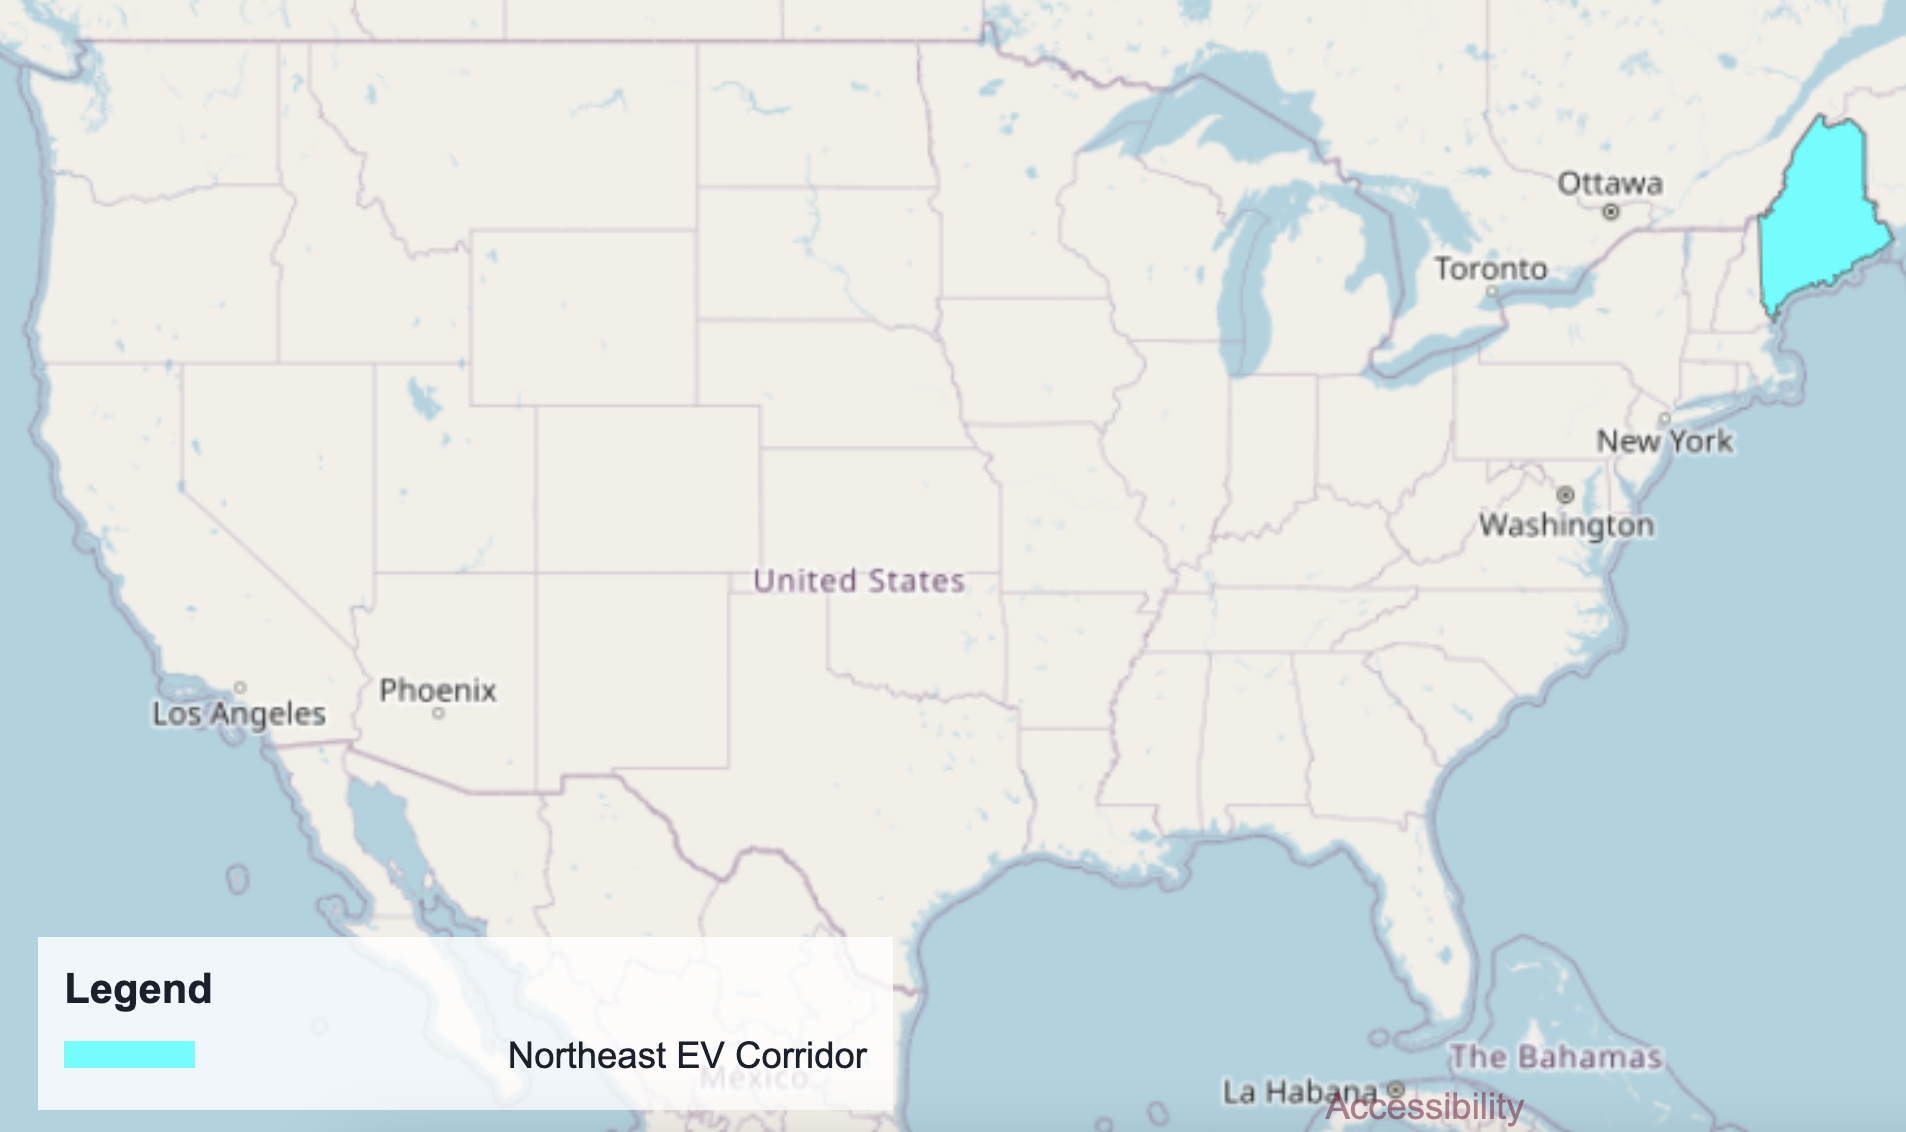
\includegraphics[width=\textwidth]{figures/northeast_ev_corridor.png}
        \caption{Northeast EV Corridor}
        \label{fig:northeast_ev_corridor}
    \end{subfigure}
    \hfill
    \begin{subfigure}[b]{0.49\textwidth}
        \centering
        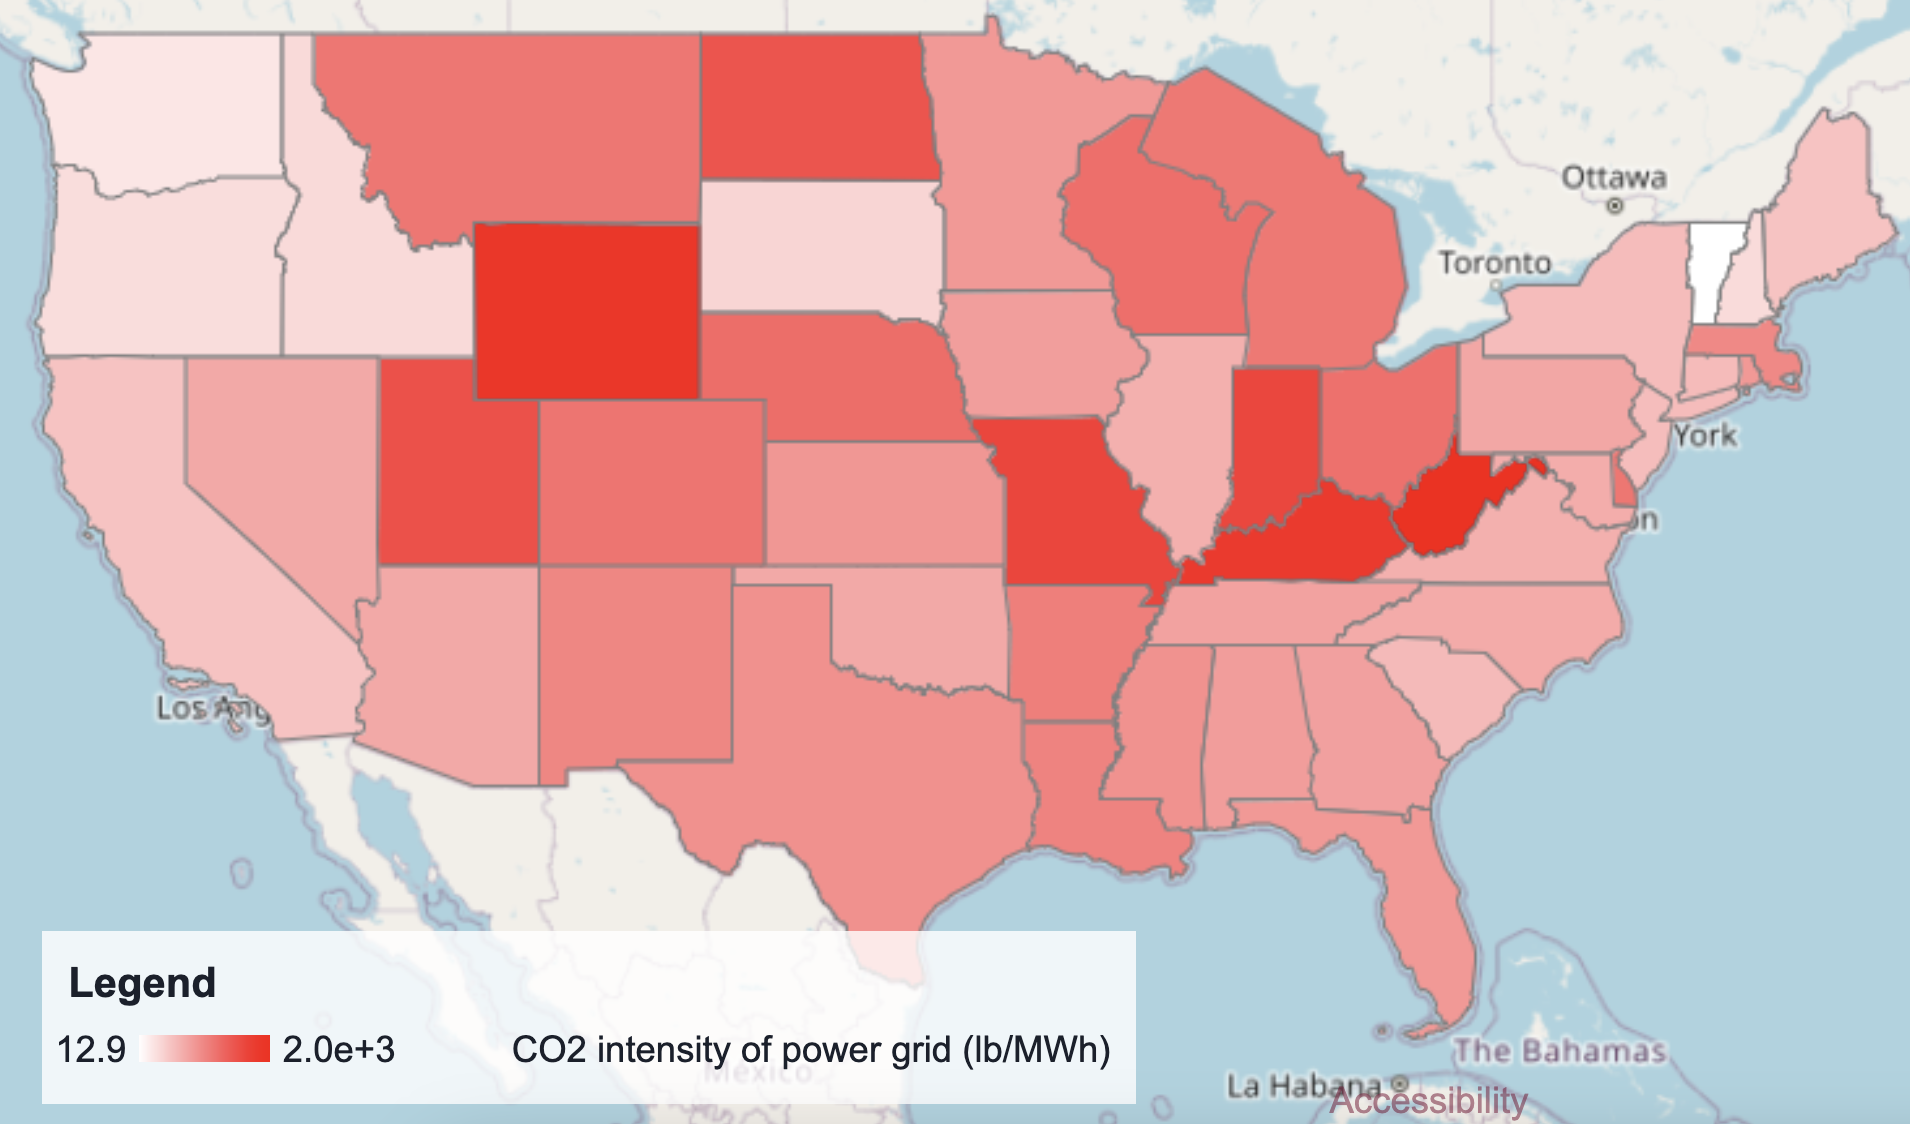
\includegraphics[width=\textwidth]{figures/grid_co2_intensity_state.png}
        \caption{Commercial electricity price by U.S. state.}
        \label{fig:grid_co2_intensity_state}
    \end{subfigure}
    \caption{Sample area features visualized with the geospatial mapping tool.}
    \label{fig:area_features}
\end{figure}

\subsubsection{Highway Features}

\textit{Highway features} represent sets of connected line features (``links") that represent the U.S. highway system. Attributes such as the annual cargo mass carried over each link can be visualized by weighting the width of each link by an amount proportional to the value of its associated attribute. Figure \ref{fig:highway_flows} illustrates the visualization of the U.S. interstate system with the tool. 

\begin{figure}[ht]
        \centering
        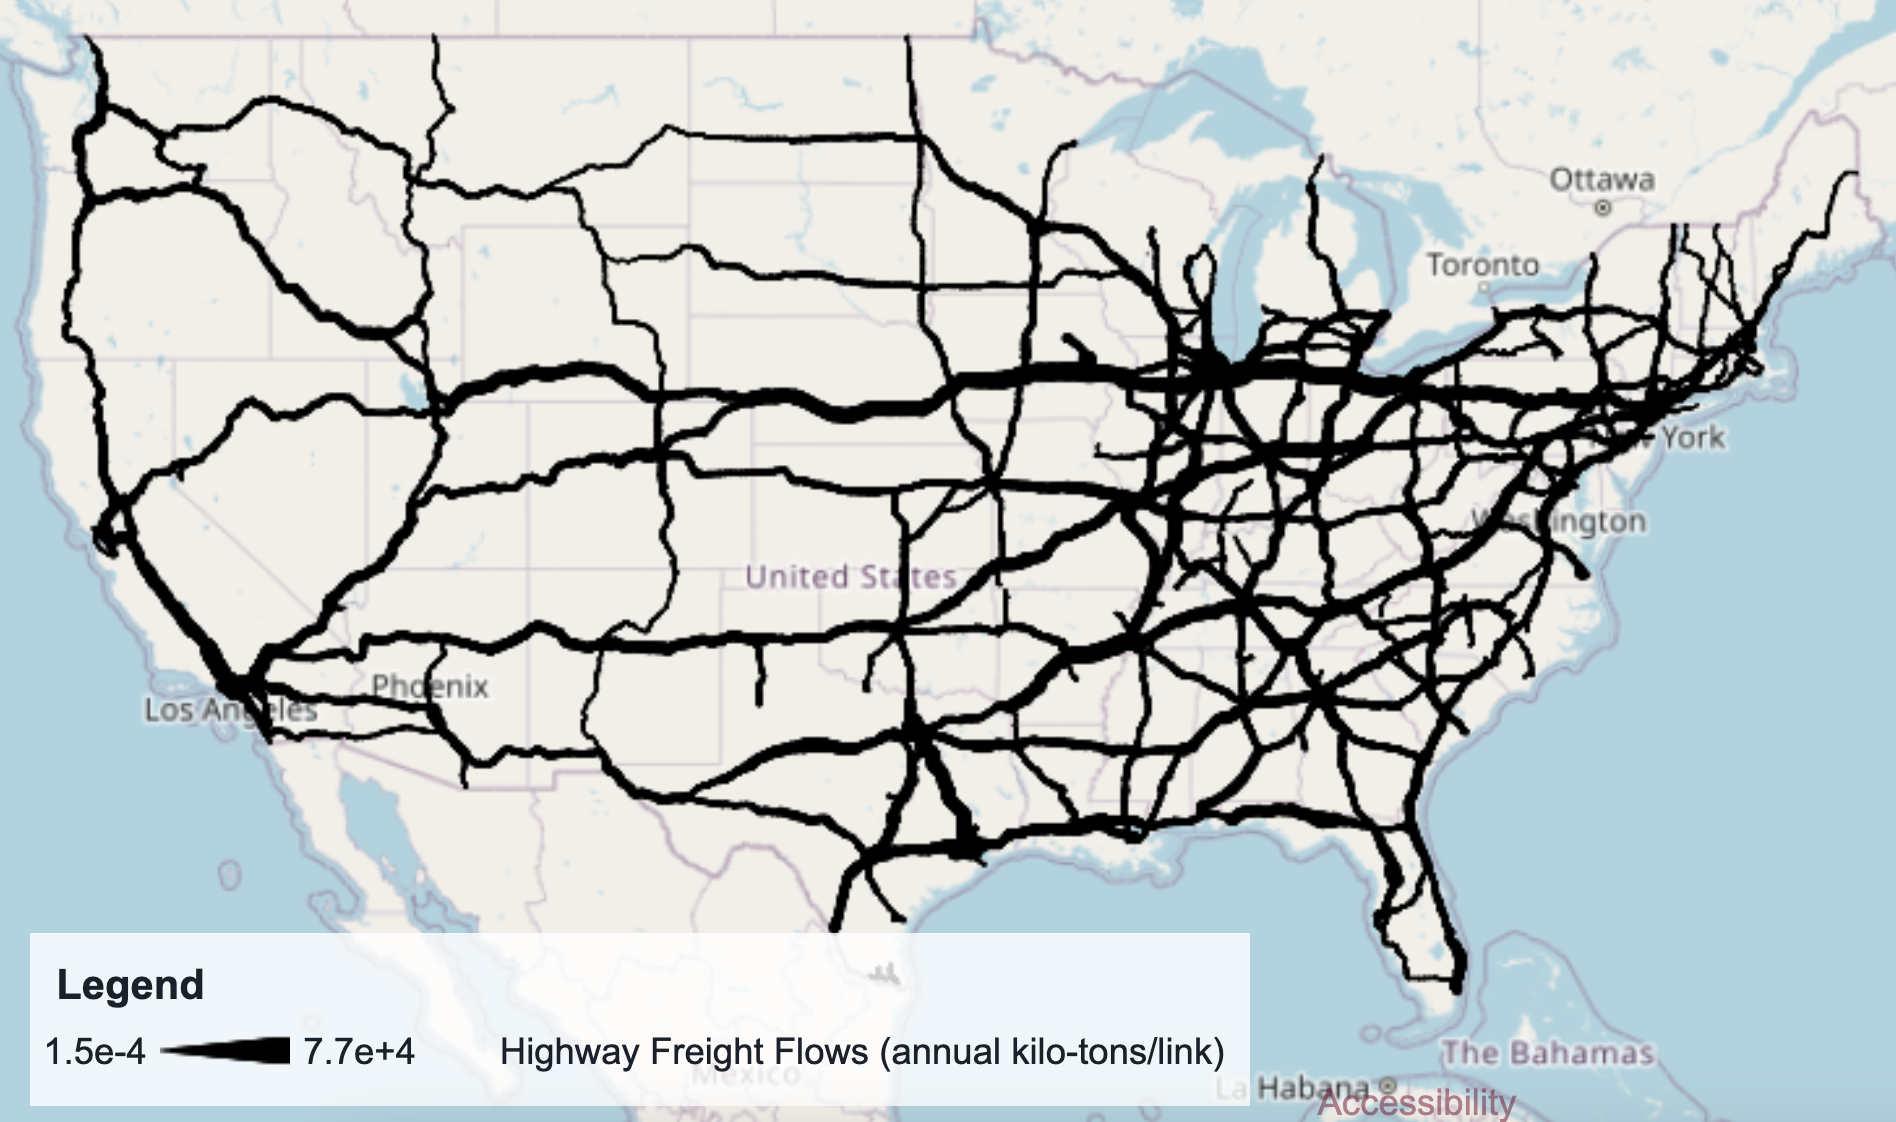
\includegraphics[width=0.7\textwidth]{figures/highway_flows.png}
        \caption{The U.S. interstate highway network, with a line width gradient used to visualize the annual cargo mass carried over each link.}
        \label{fig:highway_flows}
\end{figure}

\subsubsection{Point Features}

\textit{Point features} represent localized positions of objects on the map such as charging stations, struck stops and hydrogen production facilities. Point feature attributes, such as the installed power capacity of hydrogen production facilities, are visualized by weighting the size of each point by an amount proportional to the value of its associated attribute. Figure \ref{fig:electrolyzer_facilities} illustrates the visualization of planned and operational electrolytic hydrogen production facilities with the tool. 

\begin{figure}[ht]
        \centering
        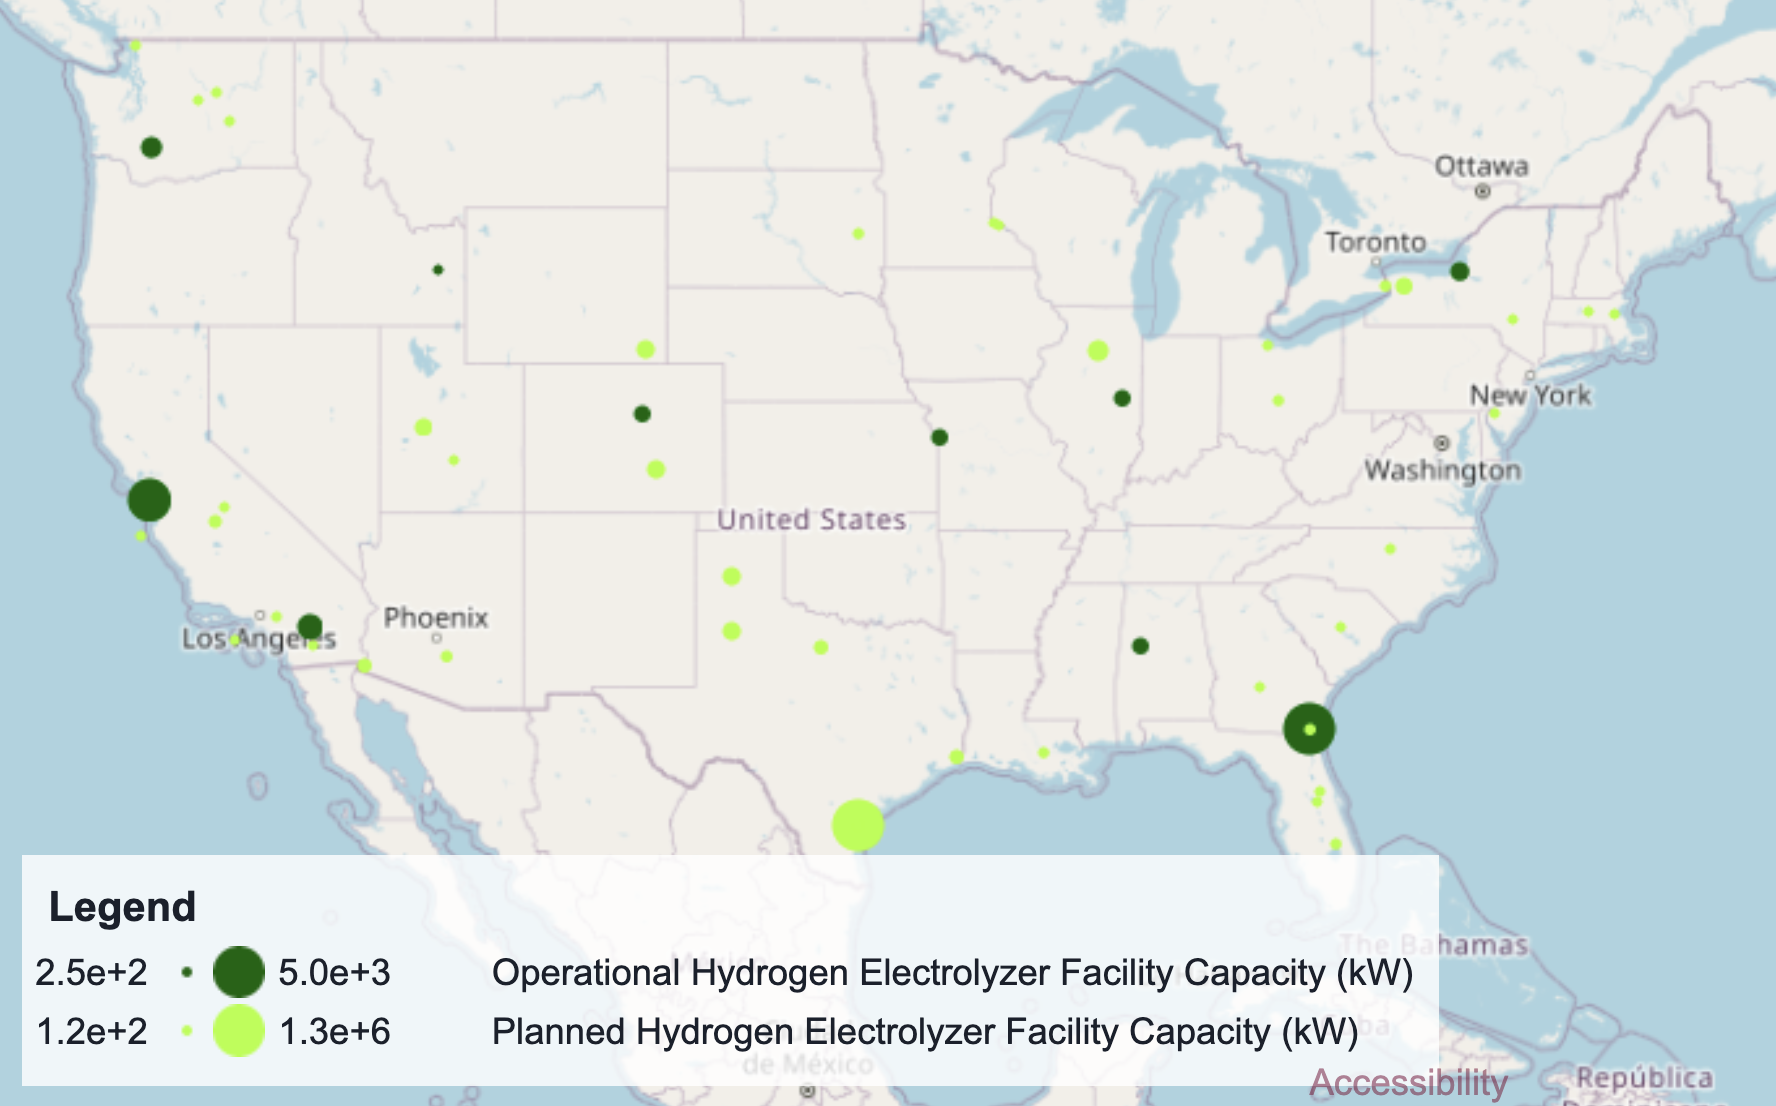
\includegraphics[width=0.7\textwidth]{figures/electrolyzer_facilities.png}
        \caption{Planned and operational electrolytic hydrogen production facilities in the U.S., with point size weighted by facility's power capacity.}
        \label{fig:electrolyzer_facilities}
\end{figure}

\subsection{Freight Flows and Associated Lifecycle Emissions}

Freight flows are visualized using data from the Freight Analysis Framework \cite{faf5_2024} maintained by the U.S. Department of State. The freight flows can be visualized either between 132 regions of the U.S., referred to as ``FAF zones", or along highways. 

\subsubsection{Highway Flows}
Flows are visualized along each highway link using one of the following two link attributes: 1) annual flow of cargo carried over the link, or 2) the number of daily trips over the link. The annual flow of cargo carried over highway links in the U.S. interstate system is shown in Figure \ref{highway_flows}.

\subsubsection{Regional Flows}
Flows between the 132 FAF zones are available for a range of modes (truck, rail, pipeline, air), but data visualized in the tool is filtered to only include freight carried by truck. The FAF5 data can be further filtered to visualize flows of specific commodities, broken down into 43 categories (cereal grains, wood products, etc.), and to visualize import and export flows separately. Regional  flows are visualized as areal densities (ton-miles per square mile) to eliminate any dependence on the sizes of origin and destination FAF5 zones. 

Figure \ref{fig:freight_flows} shows some sample visualizations of regional freight flows. 

\begin{figure}[ht]
    \centering
    \begin{subfigure}[b]{0.49\textwidth}
        \centering
        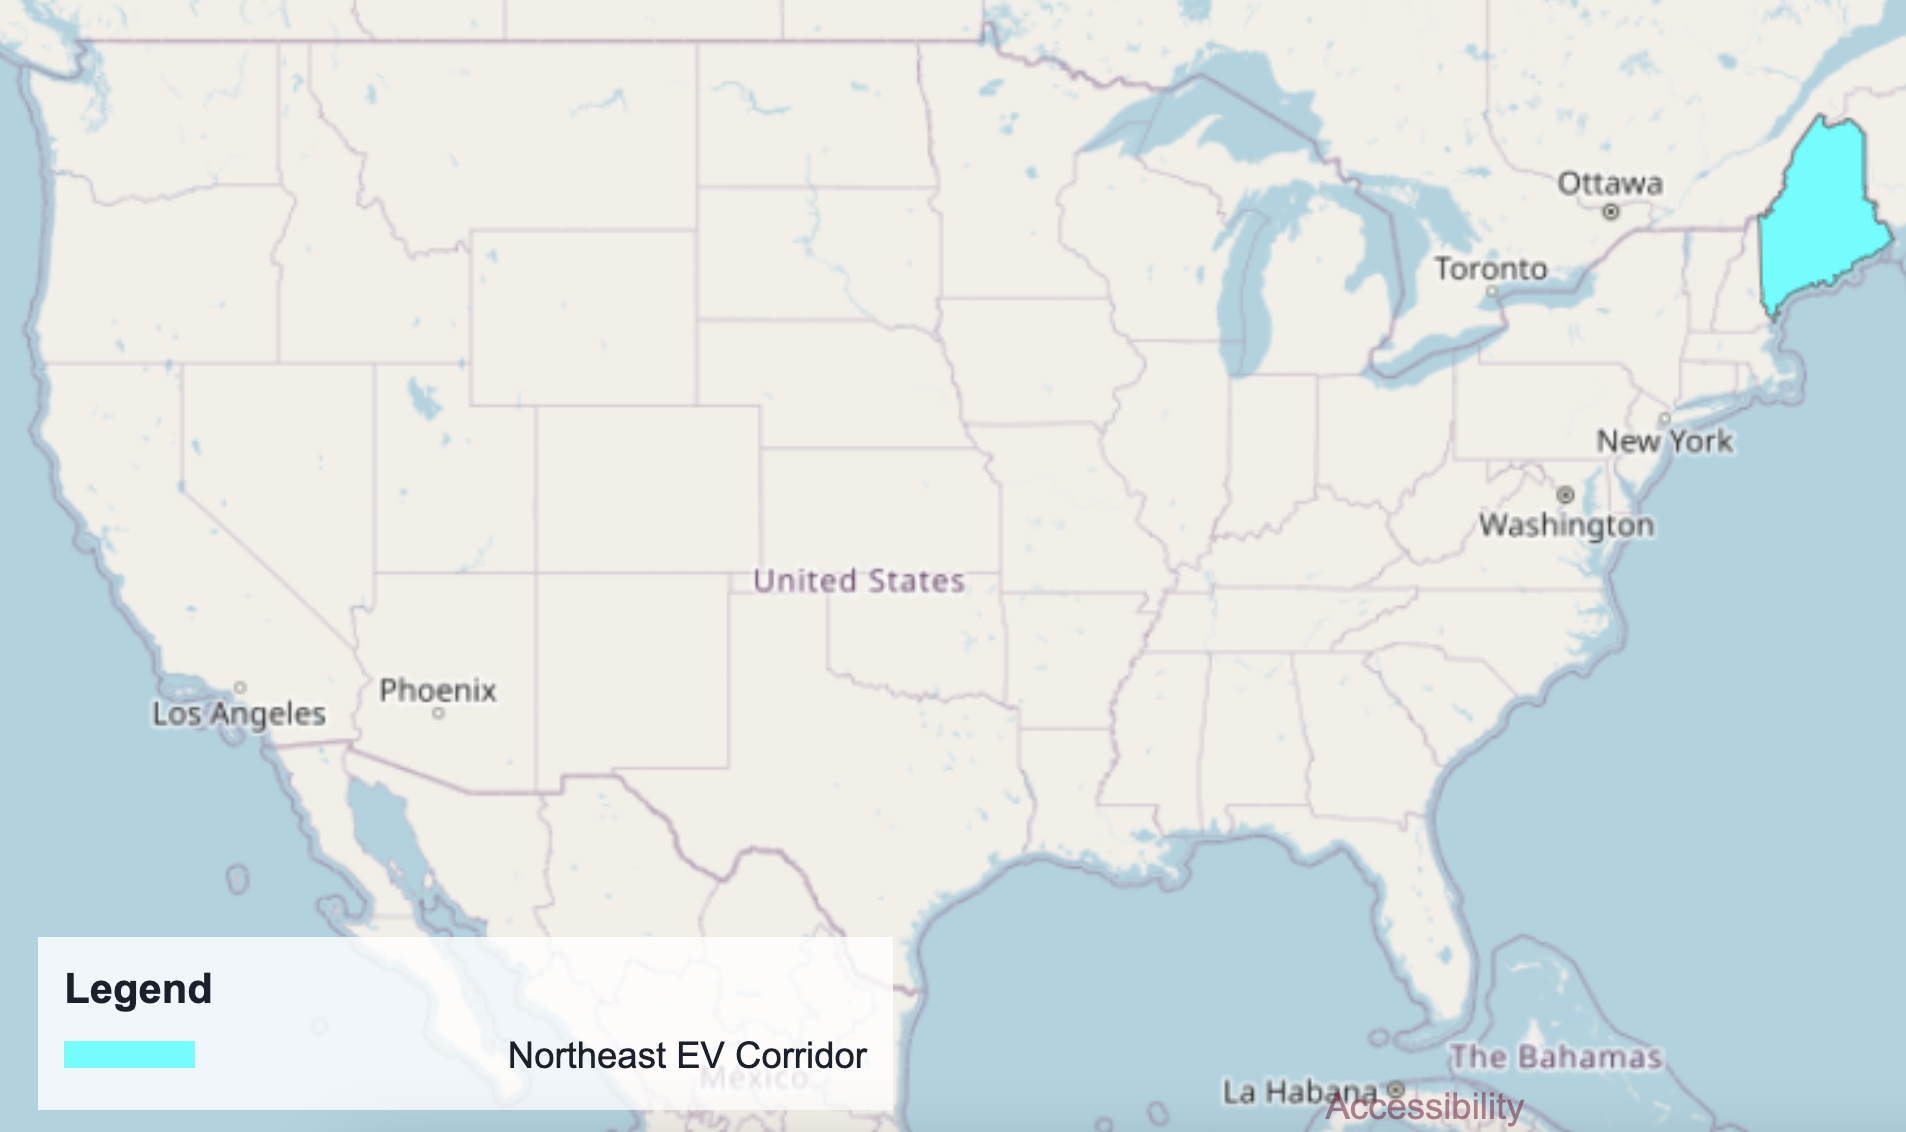
\includegraphics[width=\textwidth]{figures/northeast_ev_corridor.png}
        \caption{Northeast EV Corridor}
        \label{fig:northeast_ev_corridor}
    \end{subfigure}
    \hfill
    \begin{subfigure}[b]{0.49\textwidth}
        \centering
        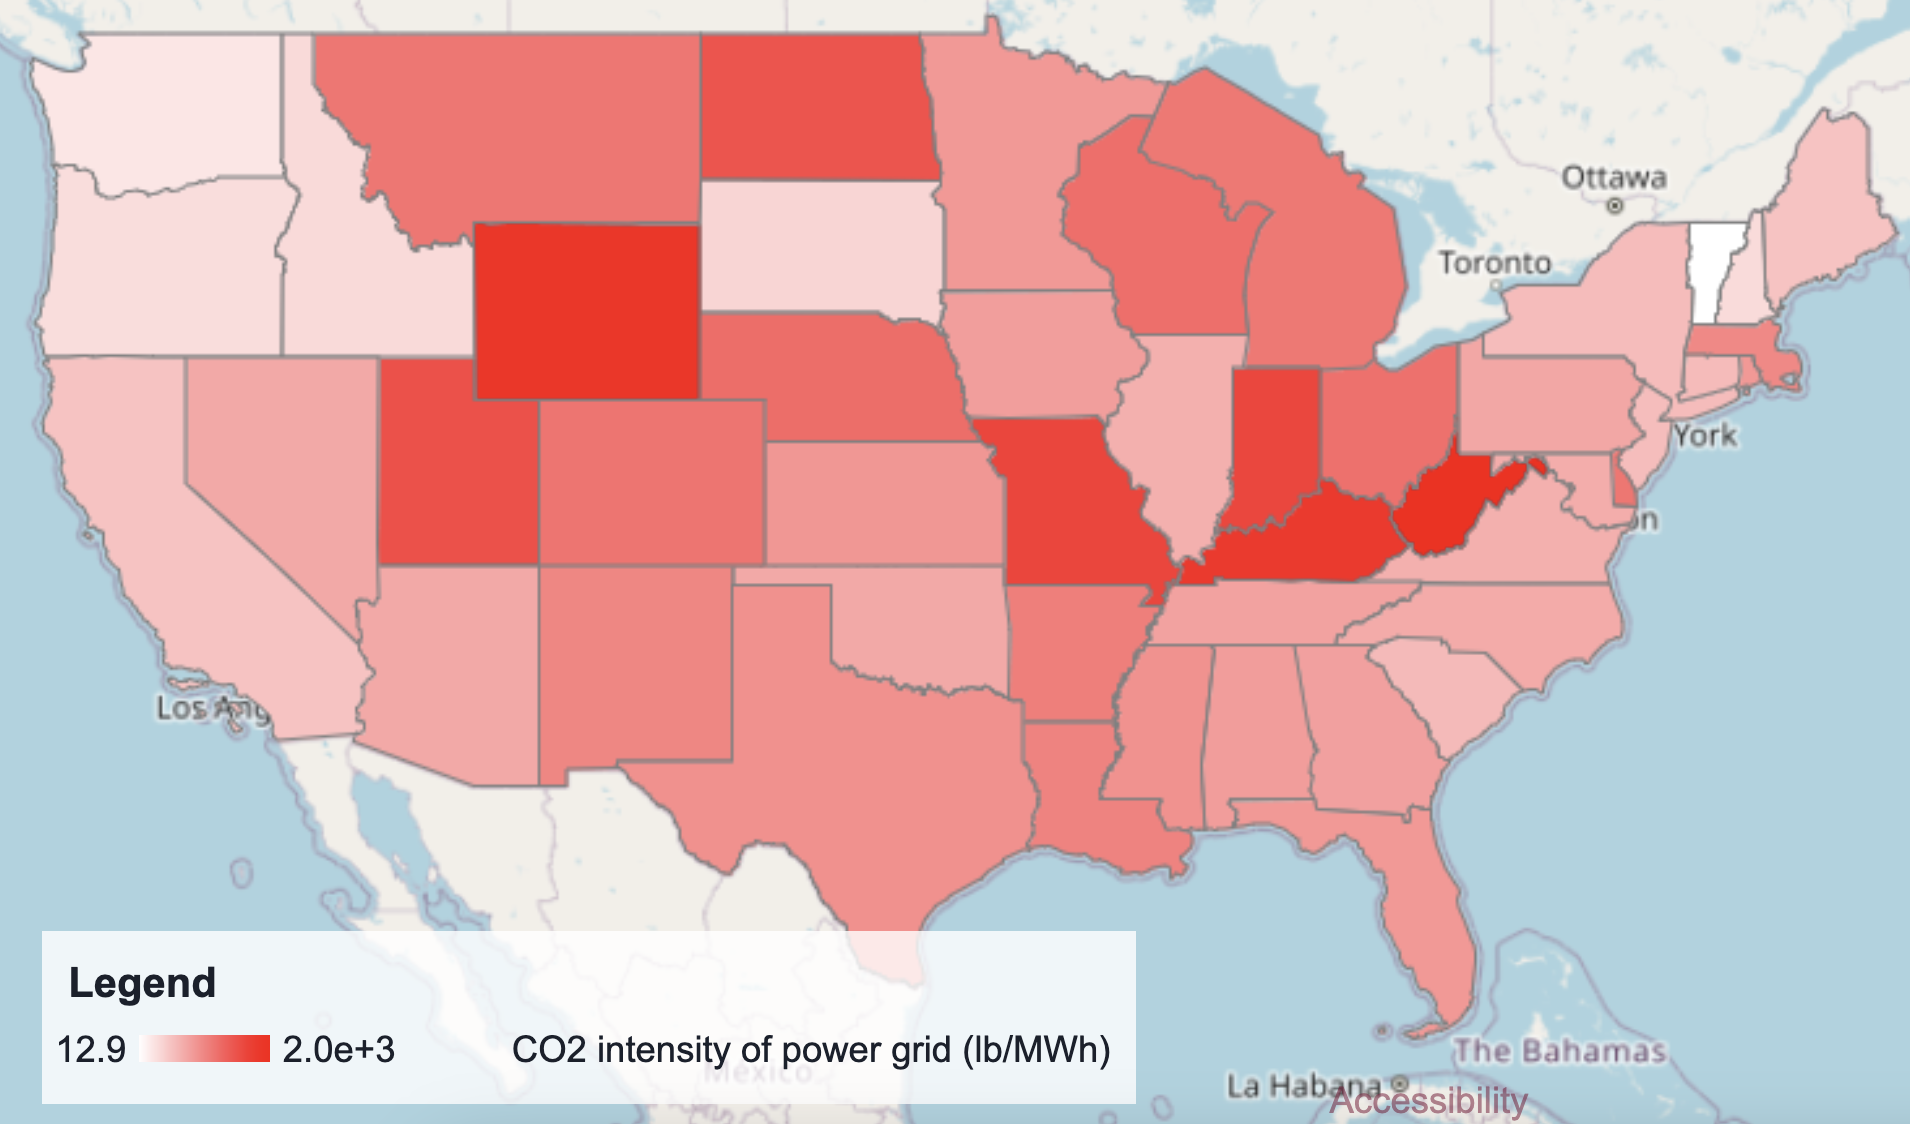
\includegraphics[width=\textwidth]{figures/grid_co2_intensity_state.png}
        \caption{Commercial electricity price by U.S. state.}
        \label{fig:grid_co2_intensity_state}
    \end{subfigure}
    \caption{Sample area features visualized with the geospatial mapping tool.}
    \label{fig:area_features}
\end{figure}

We have also developed a methodology to combine the FAF5 data with fuel production and tailpipe emission intensities from the GREET model \cite{GREET_2022} and truck characteristics and operating conditions from the 2002 Vehicle Inventory and Use Survey \cite{VIUS_2002} to evaluate approximate well-to-wheel emissions associated with interregional freight flows. Figure \ref{fig:freight_flows_emissions}

Under the current condition in which is the vast majority (>99\%) of ton-miles are carried by diesel internal combustion trucks,  emission rates are roughly proportional to freight flows. Future work is needed to investigate how the regional freight flow associated emissions change with respect to penetration of alternative energy carriers, in which case we expect regional effects (eg. the regional intensity of the electrical grid) to become more pronounced. 

Section \ref{sec:freight_flows} provides details on the methodology developed to visualize emissions associated with regional freight flows. 

\subsection{Infrastructure}

\subsection{Costs and Emissions}

\subsection{Electricity Demand and Capacity}
